\documentclass{article}
\usepackage{amsmath}
\usepackage{amsfonts}
\usepackage{array}
\usepackage{dsfont}
\usepackage{hyperref}
\usepackage{amssymb}
\usepackage{amsthm}
\usepackage{amsfonts}
\usepackage{graphicx}
% \usepackage{geometry}
\usepackage{bbold}
\usepackage{caption}
% \usepackage{pseudocode}
\usepackage{standalone}
% \usepackage[nottoc]{tocbibind}
% \usepackage{apacite}
\usepackage{etoolbox}
% \usepackage{tikz}
% \usepackage{color}
% \usepackage[T1]{fontenc}
% \usepackage{lmodern}
% \usepackage{mathptmx}
% \usepackage{standalone}
\usepackage{accents}
\usepackage{enumitem}

% used for typesetting theorem environments
\usepackage{amsthm}

% used for typesetting tikz graphs
\usepackage{tikz}
% used for typesetting automata using tikz
\usetikzlibrary{automata}

% aaron edit

\usepackage{tikz}
\usepackage{algorithmic}
\usepackage{algorithm}
\usepackage{verbatim}

% \graphicspath{ {../images/} }

\newcommand{\R}{\mathds{R}}
\newcommand{\Zplus}{\mathds{Z}_+}
\newcommand{\N}{\mathds{N}}
\newcommand{\seq}[2][j]{\left\{#2\right\}_{#1=0}^\infty}
\newcommand{\diff}[3][]{\frac{\mathrm{d}^{#1} #2}{\mathrm{d}^{#1} #3}}
\newcommand{\pdiff}[3][]{\frac{\partial^{#1} #2}{\partial^{#1} #3}}
\newcommand{\dd}{\mathrm{d}}
\newcommand{\ip}[2]{\left\langle #1,#2\right\rangle}
\newcommand{\kernl}[1]{\text{ker}(#1)}
\newcommand{\ind}[1]{\mathbb{1}_{#1}~}
\newcommand{\s}{\mathcal{S}}
\newcommand{\Sin}[1]{\sin\left(#1\right)}
\newcommand{\Cos}[1]{\cos\left(#1\right)}
\newcommand{\ubar}[1]{\underaccent{\bar}{#1}}

\newtheorem{thm}{Theorem}
\newtheorem{assmp}{Assumption}
\newtheorem{prop}{Proposition}
\newtheorem{lemma}{Lemma}

\newcolumntype{C}[1]{>{\centering\arraybackslash}p{#1}}
\newcolumntype{L}[1]{>{\raggedright\arraybackslash}p{#1}}
\newcolumntype{R}[1]{>{\raggedleft\arraybackslash}p{#1}}

\captionsetup[table]{labelfont=bf}
\captionsetup[figure]{labelfont=bf}

\title{NSERC USRA Minimal Communications Work}
\author{Willem Mueller}

\begin{document}
	\maketitle

	\section{Introduction}

		Due to advances in technology and the emergence of the Internet of things, distributed networks are becoming more pervasive across the globe. Whether they be in the home, part of an organization, or in the streets, networks are a subtle and ever-present part of modern life. With this vast and ever growing transfer of information there comes costs such as bandwidth and energy usage. The the need for minimal transfer of data thus becomes an ever more important topic. 

		Using the structure of discrete event systems we can understand what a minimal communication schema means for some supervisor, or agent in a network. A given system has event set, or alphabet $\Sigma$ and is partitioned into observable events, $\Sigma_o$ and unobservable events, $\Sigma_{uo}$. $\Sigma_o$ can be thought of as activation events of sensors that an agent has. Where as $\Sigma_{uo}$ can be thought of as events that change the system, but not directly observed by the agent. Additionally a system has a set of states $X$ and an initial state $x_0 \in X$ that are connected in a directed graph defined by transition function $\xi : X \times \Sigma \to X$. A system can thus be defined as generator $G = (X, \Sigma, \xi, x_0)$. Given $G$ let $TR(G,\Sigma)$ be all transitions of $G$ labeled with events $\Sigma$. In other words $TR(G,\Sigma) = \{(x, \sigma)\in X\times\Sigma | \xi(x, \sigma) \in X\}$. A communication schema, $COM$ is thus defined as $COM \subseteq TR(G, \Sigma_{uo})$. Let $G^*$ be the plant $G$ with $\epsilon$ transitions on all $TR(G, \Sigma)\setminus (TR(G, \Sigma_o) \bigcup COM)$. For an agent to preform it's given supervisory action it must have certain sets of states be non-indistinguishable under the information mapping $\theta : \mathcal{L}(G) \to \mathcal{L}(G^*)$ induced by $COM$. A set $M\subseteq X$ is considered non-indistinguishable \emph{iff} $\forall s \in \mathcal{L}(G)$, $\xi(x_0, \theta^{-1}(\theta(s)) \neq M$. Let $REQ \subseteq 2^X$ a subset of the power set of $X$ that specifies the state sets that must be non indistinguishable. 

		A minimum communication schema is then defined as $COM \subseteq TR(G, \Sigma_{uo})$ such that...
		\begin{enumerate}
			\item $\forall I\in\{M \in 2^X | \forall s \in \mathcal{L}(G), M = \xi^*(x_0, \theta^{-1}(\theta(s))\} $ and $ \forall r\in REQ$, $ r\nsubseteq I$
			\item $\nexists COM^* \subset COM$ such that $1.$ is satisfied
		\end{enumerate}

	\section{Discussion $\&$ Conclusion}

		The following is mainly conjecture and summery. 

		The indistinguishablity of sets is a subtle notion and ensuring that it does not occur for a given communication scheme can be difficult. Two algorithms were tested and compared. The trivial algorithm involved enumeration of states in increasing cardinality with an NFA to DFA projection to check indistinguishablity. The suffix algorithm uses a finite set of string sets to create a languages that transitions are removed from. it was found that the trivial one completed in a significantly shorter time (1ms vs 200ms). Additionally an extension of the cluster table algorithm was created that allows polynomial time computation of indistinguishablity when the set size is much less than n. This extension allows the preexisting work in acyclic plants to be applied to state sets. the extension greatly expedites the trivial algorithm so may be used to achieve a poly time computation with some sufficient conditions.

		The problem is clearly a difficult one. Broadening to all plants is clearly too general and thus leads to algorithms that will ultimately be of exponential order. However tantalizing the requirement of an acyclic plant is, this condition is far too restrictive. Almost all interesting and practical instances of DES occur with some cyclic nature. One avenue to follow would thus be sufficient conditions on plants that greatly reduce the complexity. This too may be difficult. As seen in the extension of cluster table simply checking large sets for their indestinguishablity becomes exponential, so it the requirement sets elements may need to be capped in cardinality. The best course of action would seem to be limiting the connectivity of the plant in someway, or an upper bound on the communication policy. The upper bound would ensure that the banker's sequence would terminate in non exponential time thus reducing the problem to a polynomial one. The connectivity limit seems closely related to that of the upper bound, but is somewhat open to interpretation. My sense is that the less "connected" states are to each other the less information is needed to ensure they are non-indestinguishable. Non-co-reachable or non-reachable sets could be an interesting direction too; then there is a clear decision or branching that occurred from the initial state so as to cause that structure. Therefor only those branching transitions are needed. There are many directions to go.

	\section{Work Done and Paths Followed}
		\subsection{Indistinguishablity For Sets}

			\begin{thm}
			If set $I$ is indistinguishable under some information mapping $\theta$ then any $S \subseteq I$ is indistinguishable.
			\end{thm} 

			Proof: For $I$ to be indistinguishable there exists a string $s_i$ for each state $i$ in $I$ such that some string $s = \theta (s_I)$ for all $i \in I$. it then follows that the same string $s$ could be used on any subset of $I$.

			\begin{thm}
			All strict subsets of a set $I$ being indistinguishable under some information mapping $\theta$ does not imply $I$ is indistinguishable.
			\end{thm}

			Proof: Take $I = \{1,2,3\}$. The Figure ~\ref{fig:figure1} describes a plant under some information mapping. Note that all subsets of $I$ are indistinguishable however $I$ is not.

			\begin{figure}[ht]
				\begin{minipage}[b]{\linewidth}
				\centering
				    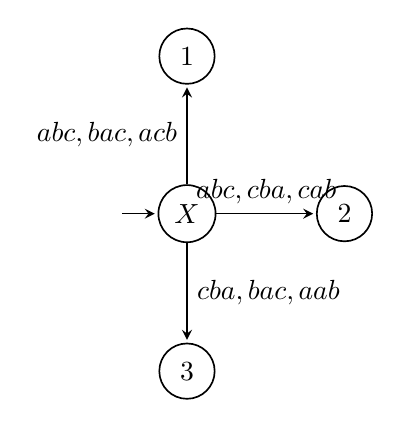
\begin{tikzpicture}[
				        >=stealth,
				        shorten >=1pt,
				        node distance=2cm,
				        auto,
				        state/.append style={minimum size=2em},
				        semithick
				        ]
				        \node[state, initial left, initial text=] (1) {$X$};
				        \node[state] (3) [right of = 1] {$2$};
				        \node[state] (2) [above of = 1] {$1$};
				        \node[state] (4) [below of = 1] {$3$};
				        \path[->]
				              (1) edge node {$abc,bac,acb$} (2)

				              (1) edge node {$abc,cba,cab$} (3)
				              
				              (1) edge node {$cba,bac,aab$} (4);
				    \end{tikzpicture}
				    \caption{Automaton $P$}
				    \label{fig:figure1}
				\end{minipage}
			\end{figure}

		\subsection{Suffix Algorithm}

			To deal with the computational complexity issue of finding a minimal communication scheme the possibility of working with a finite set of string suffixes was explored. This endeavor was however fruitless as the computational complexity was exponential and no sufficient conditions on the plant could be found that significantly reduced computation time. Additionally no rigorous proofs are added as the technique was not efficient.

			\subsubsection{Suffix Introduction}

				Generator $G$ with cycling event sequences has language, $\mathcal{L}(G)$ that is countably infinite cardinality. As a result, such a set is not feasible to work with algorithmically to test the existence of strings that result in indistinguishable state sets. It would thus be beneficial to find finite sets of strings that fully describe the plant.

				First some extra notation is required. Let $G_x$ signify the plant $G$ with the caveats that the only marked state is $x$ and a new initial state $x_\delta$ is added such that the only transition associated with $x_\delta$ is $\xi(x_\delta,\delta) = x_0$, with $\delta \notin \Sigma$ ie. $G_x = (X \bigcup \{x_\delta\}, \Sigma \bigcup \{\delta\}, \xi, x_\delta, \{x\})$. Let $S_x$ be the set of suffixes of the language accepted by $G_x$ ie. $\mathcal{L}_m(G_x)$ with length $|TR(G_x, \Sigma \bigcup \{\delta\})|$ and all strings beginning at $x_\delta$ and ending at $x$ with lengths less than $|TR(G_x,\Sigma \bigcup \{\delta\})|$.

			\subsubsection{Intersection of $S_x$ is Non-Vital}

				\begin{figure}[ht]
					\begin{minipage}[b]{\linewidth}
					\centering
					    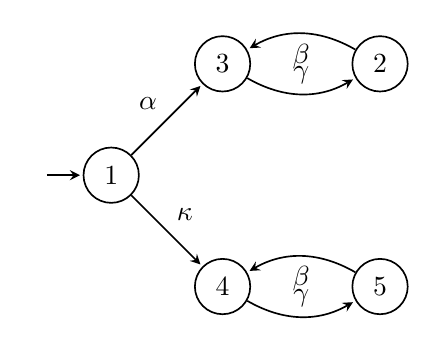
\begin{tikzpicture}[
					        >=stealth,
					        shorten >=1pt,
					        node distance=2cm,
					        auto,
					        state/.append style={minimum size=2em},
					        semithick
					        ]
					        \node[state, initial left, initial text=] (1) {$1$};
					        
					        \node[state] (2) [above right of=1] {$3$};
					        \node[state] (3) [right of=2] {$2$};
					        \node[state] (4) [below right of=1] {$4$};
					        \node[state] (5) [right of=4] {$5$};
					        \path[->]
					              (1) edge node {$\alpha$} (2)
					              (2) edge [bend right] node {$\gamma$} (3)
					              (3) edge [bend right] node {$\beta$} (2)

					              (1) edge node {$\kappa$} (4)
					              (4) edge [bend right] node {$\gamma$} (5)
					              (5) edge [bend right] node {$\beta$} (4);
					    \end{tikzpicture}
					    \caption{Automaton $P$}
					    \label{CounterExampleAutomaton}
					\end{minipage}
				\end{figure}

				Consider plant $P$ and the sets $S_3$ and $S_5$. Clearly $S_3 \bigcap S_5 \neq \emptyset$ as both sets contain the string $\gamma\beta\gamma\beta\gamma\beta\gamma$. Thus some suffixes do not impact whether or not states are non-indistinguishable. In other words for some $M \in REQ$ and $x,x' \in M$, $\forall s \in S_x$, $s$ is not necessarily unique from all $t \in S_{x'}$. The elements in $\bigcup_{x \in M} S_x$ are not needed for to ensure non-indistinguishable states.

				Take generator $G$, and $M \in REQ$.

				\begin{enumerate}
					\item Conjecture: Let $INT_M = \bigcup_{x \in M} S_x$. The elements of $INT_M$ do not impact whether or not $M$ is non-indistinguishable. 
					\item Conjecture: Let $S_{x,M} = S_x \setminus INT_M$ and $S_{x,M}^*$ be $S_{x,M}$ with the deletion of some subset of $TR(G,\Sigma_{uo})$. $\bigcap_{x \in M} S_{x,M}^* \neq \emptyset$ \emph{iff} $M$ is indistinguishable.
				\end{enumerate}

				Sketch:

				\begin{enumerate}
					\item Given $INT_M \neq \emptyset$ this implies that the string came from some over repetition of cycles of G. As the string must be of length $|TR(G,\Sigma)|$ it must not have ever visited the transition(s) that resulted in $M$ being not-indistinguishable. The Sting is thus useless as it tells us nothing of the indistinguishable nature of $M$. Therefore it may be deleted. See automation $P$.

					\item Clearly $\bigcap_{x \in M} S_{x,M}^* = \emptyset$ $\implies$ $M$ is non-indistinguishable. As $S_{x,M}^*$ visits all reachable transitions of $G$ the only stings not contained in $S_{x,M}^*$ are those which simply have mass repletion of cycles. Thus we see all requisite information in $S_{x,M}^*$ and therefore $M$ being non-indistinguishable $\implies$ $\bigcap_{x \in M} S_{x,M}^* = \emptyset$.  \emph{sorry soooo rough}
				\end{enumerate} 


			\subsubsection{Algorithm} 

				%\begin{algorithm}
				%\caption{
				Calculate $COM$, given some generator $G$ and non-indistinguishable state-set requirement $REQ$
				%}
				%\label{minCOM}
				\begin{algorithmic}[5]
					\STATE $G \leftarrow AddStartTrans(G)$
					\STATE $COM \leftarrow TR(G,\Sigma_{uo})$
					\FORALL{$M \in REQ$}
						\FORALL{$x \in M$}
							\IF{x has not been seen before}
								\STATE $S_x \leftarrow BuildSuffixSet(x, G)$
							\ENDIF
						\ENDFOR
						\STATE $INT_M \leftarrow \bigcap_{x \in M} S_x$
						\FORALL{$x \in M$}
							\STATE $S_{x,M} \leftarrow S_x \setminus INT_M$
						\ENDFOR
					\ENDFOR
					\FORALL{$\sigma \in TR(G,\Sigma_{uo})$}
						\FORALL{$M \in REQ$}
							\FORALL{$x \in M$}
								\STATE $S_{x,M}^* \leftarrow S_{x,M}$
								\FORALL{$s \in S_{x,M}^*$}
									\STATE $s \leftarrow EventSubtraction(s, \sigma)$
								\ENDFOR
							\ENDFOR
							\IF{$\bigcap_{x \in M} S_{x,M}^* = \emptyset$}
								\STATE $COM \leftarrow COM \setminus \{\sigma\}$
								\FORALL{$x \in M$}
									\STATE $S_{x,M} \leftarrow S_{x,M}^*$
								\ENDFOR
							\ENDIF
						\ENDFOR
					\ENDFOR
					\RETURN $COM$
				\end{algorithmic}
				%\end{algorithm}

				\begin{comment}
				\begin{enumerate}
					\item let $COM$ be equal to $TR(G,\Sigma_{uo})$.
					\item $\forall M \in BAD $ 
					\begin{enumerate}
						\item $\forall x \in M$
						\begin{enumerate}
							\item build $S_x$ by following all paths entering $x$.
						\end{enumerate}
						\item Remove $\bigcap_{x\in M} S_x$ from each $S_x$ for $x\in M$
					\end{enumerate}
					\item $\forall \sigma \in TR(G,\Sigma_{uo})$
					\begin{enumerate}
						\item Remove $\sigma$ from all $s \in S_x$ for each $S_x$
						\item Compare all $s$ in each $S_x$.
						\begin{enumerate}
							\item If $\bigcap_{x\in M} S_x = \emptyset$ delete $\sigma$ from $COM$.
							\item Else do nothing.
						\end{enumerate}
					\end{enumerate}
					\item return COM.
				\end{enumerate}
				\end{comment}


		\subsection{Worked Example}

			Consider the automaton $G = (\{1, 2, 3, 4\}, \{a, b, c\}, \xi, \{1\})$ where $\xi$ is depicted in Figure \ref{CounterExampleAutomaton}.

			\begin{figure}[ht]
			\begin{minipage}[b]{\linewidth}
			\centering
			    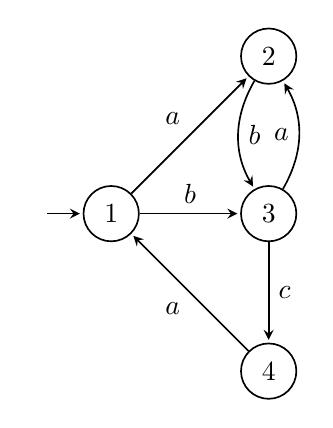
\begin{tikzpicture}[
			        >=stealth,
			        shorten >=1pt,
			        node distance=2cm,
			        auto,
			        state/.append style={minimum size=2em},
			        semithick
			        ]
			        \node[state, initial left, initial text=] (1) {$1$};
			        
			        \node[state] (3) [right of=1] {$3$};
			        \node[state] (2) [above of=3] {$2$};
			        \node[state] (4) [below of=3] {$4$};
			        \path[->]
			              (1) edge node {$a$} (2)
			              (1) edge node {$b$} (3)

			              (4) edge node {$a$} (1)
			              (2) edge [bend right] node {$b$} (3)
			              (3) edge [bend right] node {$a$} (2)

			              (3) edge node {$c$} (4);
			    \end{tikzpicture}
			    \caption{Automaton $G$}
			    \label{CounterExampleAutomaton}
			\end{minipage}
			\end{figure}

			Suppose $\Sigma_o = \{a\}$, $\Sigma_{uo} = \{b, c\}$.
			Suppose $BAD = \{ \{2, 4\} \}$.

			The following demonstrates how your proposed algorithm operates on this example.

			\begin{enumerate}
			    \item[Alg Step 1.] Let $COM = TR(G, \Sigma_{uo}) = \{(1, b)\}$.
			    \item[Alg Step 2.] Let $M = \{2, 4\}$ where $\{2, 4\} \in BAD$.
			    \begin{enumerate}
			        \item[Alg Step 2.(a)] $S_2 = \{a, bcaa, cabcaa, ababa, aababa, aba, bcaaba, ba, bcaba, abcaba\}$,\\$S_4 = \{bc, bcabc, abcabc, ababc, aababc, bababc, babc, cababc, abc, bcaabc\}$
			        \item[Alg Step 2.(b)]
			            \begin{itemize}
			                \item
			                    $\bigcap_{x \in M} S_x = S_2 \cap S_4 = \emptyset$
			                \item $S_2 = S_2 \setminus \bigcap_{x \in M} S_x = S_2$
			                \item $S_4 = S_4 \setminus \bigcap_{x \in M} S_x = S_4$
			            \end{itemize}
			    \end{enumerate}
			    \item[Alg Step 3. (First Time)] Let $\sigma = (1, b)$ where $(1, b) \in TR(G, \Sigma_{uo})$.
			    \begin{enumerate}
			        \item[Alg Step 3.(a)]
			            Remove each occurrence of $b$ corresponding to transition $\sigma$ from all $s \in S_2$.
			            The result is $S_2 = \{a, caa, cacaa, aabcaa, ababa, aababa, aba, caaba, a, caba, abcaba, acaba\}$.

			            Remove each occurrence of $b$ corresponding to transition $\sigma$ from all $s \in S_4$.
			            The result is $S_4 = \{c, cac, abcabc, acac, abcac, abac, aabac, babac, bac, cabac, ac, caabc\}$.
			        \item[Alg Step 3.(b)]
			            Compare all $s$ in $S_x$
			        \begin{enumerate}
			            \item[Alg Step 3.(b).i.]
			                Delete $(1, b)$ from $COM$ since $\bigcap_{x \in M} S_x = S_2 \cap S_4 = \emptyset$.
			                The result is $COM = COM \setminus \{(1, b)\} = \{(2,b), (3,c)\}$.
			        \end{enumerate}
			    \end{enumerate}
			    \item[Alg Step 3. (Second Time)] Let $\sigma = (2, b)$ where $(2, b) \in TR(G, \Sigma_{uo})$.
			    \begin{enumerate}
			        \item[Alg Step 3.(a)]
			            Remove each occurrence of $b$ corresponding to transition $\sigma$ from all $s \in S_2$.
			            The result is $S_2 = \{a, caa, cacaa, aacaa, aaa, aaaa, aa, caaa, a, caa, acaa, acaa\}$.

			            Remove each occurrence of $b$ corresponding to transition $\sigma$ from all $s \in S_4$.
			            The result is $S_4 = \{c, cac, acac, acac, acac, aac, aaac, aac, ac, caac, ac, caabc\}$.
			        \item[Alg Step 3.(b)]
			            Compare all $s$ in $S_x$
			        \begin{enumerate}
			            \item[Alg Step 3.(b).i.]
			                Delete $(2, b)$ from $COM$ since $\bigcap_{x \in M} S_x = S_2 \cap S_4 = \emptyset$.
			                The result is $COM = COM \setminus \{(2, b)\} = \{(3,c)\}$.
			        \end{enumerate}
			    \end{enumerate}
			    \item[Alg Step 3. (Third Time)] Let $\sigma = (3, c)$ where $(3, c) \in TR(G, \Sigma_{uo})$.
			    \begin{enumerate}
			        \item[Alg Step 3.(a)]
			            Remove each occurrence of $c$ corresponding to transition $\sigma$ from all $s \in S_2$.
			            The result is $S_2 = \{a, aa, aaa, aaaa,\}$.

			            Remove each occurrence of $c$ corresponding to transition $\sigma$ from all $s \in S_4$.
			            The result is $S_4 = \{\epsilon, a, aa, aaa\}$.
			        \item[Alg Step 3.(b)]
			            Compare all $s$ in $S_x$
			        \begin{enumerate}
			            \item[Alg Step 3.(b).i.]
			                Keep $(3, c)$ from $COM$ since $\bigcap_{x \in M} S_x = S_2 \cap S_4 = \{a, aa, aaa\}$.
			                The result is $COM = \{(3,c)\}$.
			        \end{enumerate}
			    \end{enumerate}
			    \item[Alg Step 4.] Return $COM = \{(3,c)\}$.
			\end{enumerate}

			Having computed $COM$, automaton $G\ast$ is defined in Figure \ref{CounterExampleAutomatonGStar}.
			Then map $\theta : \mathcal{L}(G) \rightarrow \mathcal{L}(G\ast)$ is defined from $G\ast$ and $BAD$ is satisfied.

			\begin{figure}[ht]
			\begin{minipage}[b]{\linewidth}
			\centering
			    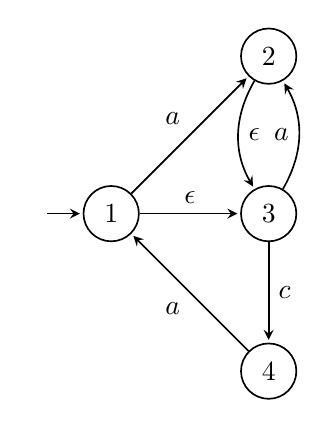
\begin{tikzpicture}[
			        >=stealth,
			        shorten >=1pt,
			        node distance=2cm,
			        auto,
			        state/.append style={minimum size=2em},
			        semithick
			        ]
			        \node[state, initial left, initial text=] (1) {$1$};
			        \node[state] (3) [right of=1] {$3$};
			        \node[state] (2) [above of=3] {$2$};
			        \node[state] (4) [below of=3] {$4$};
			        \path[->]
			              (1) edge node {$a$} (2)
			              (1) edge node {$\epsilon$} (3)
			              (4) edge node {$a$} (1)
			              (2) edge [bend right] node {$\epsilon$} (3)
			              (3) edge [bend right] node {$a$} (2)
			              (3) edge node {$c$} (4);
			    \end{tikzpicture}
			    \caption{Automaton $G\ast$}
			    \label{CounterExampleAutomatonGStar}
			\end{minipage}
			\end{figure}


		\subsection{Trivial Algorithm}
			Given some requirement of non-indistinguishable sets $REQ$ and a plant $G$.

			\begin{algorithmic}[5]
				\STATE $i=1$
				\WHILE{$i \leq  2^{|TR_u(G)|}$}
					\STATE $TR_u^* \leftarrow ithBankersSet(i,TR_u(G))$
					\STATE $Indes \leftarrow NFAtoDFA(TR_u^*,G)$
					\IF{$Indes \bigcap REQ = \emptyset$}
						\RETURN $TR_u^*$
					\ENDIF
					\STATE $i \leftarrow i + 1$
				\ENDWHILE
				\RETURN $TR(G)$
			\end{algorithmic}

			This algorithm functions by first enumerating all subsets of unobserved transitions $TR_u(G)$. It then applies the NFA to DFA projection to the NFA created by replacing all elements of $TR_u(G) \setminus TR_u^*$ with those of $\epsilon$-transitions. the state sets resulting from the projection are then used to determine indistinguishablity of the sets and whether $REQ$ is satisfied. Minimality is achieved as the bankers sequence enumerates in order of cardinality from least to greatest and thus the fist solution found is minimal. 

			The computational complexity is at worst case, $2^{|X|(|\Sigma|+1)}$. The number of subsets of $TR_u(G)$ is at most $2^{|X\times\Sigma|}$ and therefor the while loop at worst case is of the same order. Within the loop the greatest complexity step it the NFA to DFA and is order $2^{|X|}$. The total complexity is thus $2^{|X|(|\Sigma|+1)}$.

		\subsection{Edge Cut Method}
			Given a plant $G$ and some requirement of non-indistinguishable sets $REQ$. With the additional constraints that $A \bigcap B = \emptyset$ for all $A,B\in REQ$ and for each $M\in REQ$ there exists a state in $M$ such that no entering transition is observed.

			\begin{algorithmic}[5]
				\STATE $States \leftarrow \emptyset$
				\FORALL{ $M \in REQ$}
					\FORALL{ $X \in M$ }
						\IF{$X$ has no observed entering transitions AND $X$ has fewer transitions than any previous element}
							\STATE $X^* \leftarrow X$
						\ENDIF
					\ENDFOR
					\STATE $States \leftarrow States \bigcup \{X^*\}$
				\ENDFOR
				\RETURN TrivialAlgorithm($G$, $REQ$, $TR(States)$)
			\end{algorithmic}

		\subsection{NFA to DFA Computation}
			\begin{thm}
			If plant $G$ has only unique transition labels then the NFA to DFA projection is linear with any number of $\epsilon$ exchanges.
			\end{thm} 

			Proof: As the terminating event $\sigma \in \Sigma$ is unique for every string $s \in L_\theta(G)$ regardless of the information mapping $\theta : L(G) \rightarrow L_\theta(G)$, every $s$ can only lead to state sets where they are the $\epsilon$ reach from the state with $\sigma$ entering.

			\begin{thm}
			For some plant $G$ under information mapping $\Theta: G \rightarrow G_\Theta$, let the state space of $G_\Theta$ under the NFA to DFA be $Q$. If $|TR(G_\Theta)| <= n - 1$ then $|Q| <= 2^{|TR(G_\theta)|+1}$ otherwise $|Q| <= 2^n$
			\end{thm}

			Proof: if $|TR(G_\theta))| < n$ then the largest connected graph that can be made in the NFA is of size $|TR(G_\theta)|+1$ and that implies that there are at most $|TR(G_\theta)|+1$ clusters in $G_\theta$. Therefore the DFA will have size less then or equal to $2^{|TR(G_\theta)|+1}$.

		\section{Extension of Weilin Wang and Lafortune Cluster Table}
			\subsection{Intro and Changes}
				In a very broad sense this algorithm functions by creating larger clusters to compare to. This is achieved by taking sets of clusters opposed to individual ones. the reasoning behind this is that knowing cluster pairs are indistinguishable does not imply larger sets are indistinguishable as a result the indistinguishable of k-cluster sets must but be known.

				First the idea of a cluster, $\phi \in \Phi$ is required. Let $c : X \rightarrow \Phi$, $c(x)$ and is defined $\forall x\in X$ such that $x$ has at least observable in-degree 1. $c(x)$  is the set of all states $x'\in X$ such that $x'$ is reachable by $\epsilon$-transitions or $x' = x$. 
				
				Second the the mapping $R: 2^\Phi \times \Sigma \rightarrow 2^\Phi$ is needed. Thus for $\Psi \subseteq \Phi$ and $\sigma \in \Sigma$, $R(\phi,\sigma)$ is the set of clusters reachable by $\sigma$ from the clusters of $\Psi$.

				let $M$ be a mapping $\Phi\times\phi^{K-1} \rightarrow \{1,0\}$ simply used to indicate that the set of $\phi_i\bigcup\Psi$ has been explored.$\\$


				Given some plant $G$ and tuple size $K$:

				\begin{algorithmic}[5]
					\STATE $\Phi \leftarrow constructClusterSet(G)$
					\STATE $T \leftarrow constructTable(\Phi)$
					\STATE note: $T$ is initiated wit all $\phi_i$ already added to their lists and given a value 0 for the function $M: \phi^K \rightarrow \{1,0\}$
					\WHILE{$\exists M(\phi_i,\Psi) = 0$}
						\STATE note: $|\Psi| < K$ and is the elements of each $\phi_i$ list in $T$
						\STATE pick a $\phi_i$ and $\Psi$ such that $M(\phi_i,\Psi) = 0$
						\FORALL{ $\sigma \in \Sigma$ }
							\STATE add the subsets $R(\phi_i\bigcup\Psi,\sigma)$ to the lists in $T$
						\ENDFOR
						\STATE $M(\phi_i,\Psi) \leftarrow 1$ 
					\ENDWHILE

					\RETURN indistinguishableSetsSizeK($T$,$K$)
				\end{algorithmic}

			\subsection{Complexity}
				The cardinality of $\Phi$ is clearly less than or equal to $|X|$.

				The table can have a maximal number of entries per line of $\Sigma_{i=1}^{K-1} {{|X|}\choose{i}}$.

				Thus the table has $O(|X| \times |X|^{K-1}) = |X|\times |\Sigma_{i=1}^{K-1}| {{|X|}\choose{i}}$

				therefore computing the while loop is $O(|X|^K \times |X|^K \times|\Sigma|)$

				the additional $|X| \times |X|^{K-1} \times|\Sigma|$ comes from the for loop and then the creation of size $K-1$ subsets of the $\sigma$ reach and the second $|X|$ is a result from possibly having to add them to each row.

			\subsection{Worked Example}
				Given plant $G$, find all tuples of indistinguishable states size 3 or smaller.

				\begin{figure}[ht]
					\begin{minipage}[b]{\linewidth}
					\centering
					    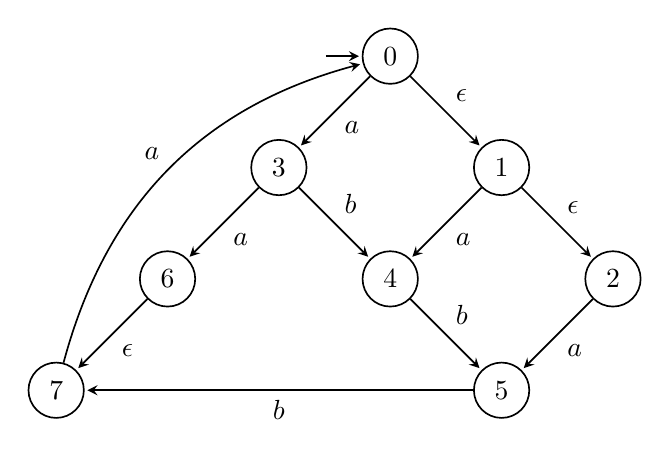
\begin{tikzpicture}[
					        >=stealth,
					        shorten >=1pt,
					        node distance=2cm,
					        auto,
					        state/.append style={minimum size=2em},
					        semithick
					        ]
					        \node[state, initial left, initial text=] (1) {$0$};
					        
					        \node[state] (2) [below right of=1] {$1$};
					        \node[state] (3) [below right of=2] {$2$};
					        \node[state] (4) [below left of=1] {$3$};
					        \node[state] (5) [below right of=4] {$4$};
					        \node[state] (6) [below right of=5] {$5$};
					        \node[state] (7) [below left of=4] {$6$};
					        \node[state] (8) [below left of=7] {$7$};
					        \path[->]
					              (1) edge node {$a$} (4)
					              (2) edge node {$a$} (5)
					              (4) edge node {$a$} (7)
					              (3) edge node {$a$} (6)
					              (8) edge [bend left] node {$a$} (1)

					              (4) edge node {$b$} (5)
					              (5) edge node {$b$} (6)
					              (6) edge node {$b$} (8)
					            
					              (1) edge node {$\epsilon$} (2)
					              (2) edge node {$\epsilon$} (3)
					              (7) edge node {$\epsilon$} (8);
					    \end{tikzpicture}
					    \caption{Automaton $G$}
					    \label{CounterExampleAutomaton}
					\end{minipage}
				\end{figure}

				Begin by creating $\Phi$. $\Phi$ is the set of all clusters of $G$. Enumerate through all $x \in X $ of $G$ checking if $x$ has any observed transitions entering it. For those $x$'s that do; find all states that can be reached from $x$ by $\epsilon$ transitions. The set of $x$ and all states that are $\epsilon$ reachable is a cluster, so add that to $\phi$. The start state is considered to have an implicit entering transition. Additionally for convention name the start state cluster $\phi_0$. I the example, the cluster $\phi_0$ is the set of states reachable by $\epsilon$-transitions from state $0$. Thus $\phi_0 = \{0,1,2\}$ and the rest of the clusters can be seen in Table ~\ref{tab:table1}.

				Next the actual cluster table, T must be instantiated. This is done by creating a table with the first column containing each cluster. Then the same clusters are added to the second column lists and the $M$ function value is assigned a 0 indicating that is has not been checked. the initailization of the table is now complete and can be seen in Table ~\ref{tab:table2}.

				Following instantiation, for the first appearance of $M(\phi_i,\{\phi\}) = 0$ follow all transitions of a out of $\phi_i\bigcap\{\phi\}$. In this example the first instance is $M(\phi_0,\phi_0) = 0$ so following all transitions of type $a$ it is found that the reach is $\{\phi_3,\phi_4,\phi_5\}$. All subsets are then taken of this set and added to their respective lists as seen in the following table. Transition $b$ is then followed and the resulting reach from $\phi_0$ is $\emptyset$, so no action is taken. Lastly $M(\phi_0,\phi_0)$ is changed to 1. the resulting change to T can be seen in Table ~\ref{tab:table3}.

				In the second iteration no new indistinguishable objects are found so there is no change other than the indication of the $M$ function as seen in Table ~\ref{tab:table4}.

				In the fifth iteration $M(\phi_3,\phi_4)$ is set to 1 and so is $M(\phi_4,\phi_3)$ as the check is the same for each and thus does not need to be repeated. this is shown in Table ~\ref{tab:table7}

				After the thirteenth iteration all $M$ function values are 1, so the table is then converted from indistinguishable clusters to to indistinguishable states of up to three entries. The algorithm then outputs Indistinguishable States. In the example this output would be: $\{\{0,1,2\},\{0,1\},\{0,2\},\{1,2\},\{3,4,5\},\{3,4\},\{3,5\},\\\{4,5\},\{4,5,7\},\{4,7\},\{5,7\},\{6,7\}\}$.



				\begin{table}[h!]
				  \begin{center}
				    \caption{$\Phi$, the Clusters of $G$}
				    \label{tab:table1}
				    \begin{tabular}{r|l}
				      Cluster & Element\\
				      \hline
				      $\phi_0$ & 0, 1, 2\\
				      $\phi_1$ & 6, 7\\
				      $\phi_2$ & 7\\
				      $\phi_3$ & 3\\
				      $\phi_4$ & 4\\
				      $\phi_5$ & 5\\
				    \end{tabular}
				  \end{center}
				\end{table}


				\begin{table}[h!]
				  \begin{center}
				    \caption{T initial}
				    \label{tab:table2}
				    \begin{tabular}{r|l|l}
				      Cluster & indistinguishable Sets & $M(\phi_i, \{\phi\})$\\
				      \hline
				      $\phi_0$ & $\phi_0$ & 0\\
				      $\phi_1$ & $\phi_1$ & 0\\
				      $\phi_2$ & $\phi_2$ & 0\\
				      $\phi_3$ & $\phi_3$ & 0\\
				      $\phi_4$ & $\phi_4$ & 0\\
				      $\phi_5$ & $\phi_5$ & 0\\
				    \end{tabular}
				  \end{center}
				\end{table}


				\begin{table}[h!]
				  \begin{center}
				    \caption{T iteration 1}
				    \label{tab:table3}
				    \begin{tabular}{r|l|l}
				      Cluster & indistinguishable Sets & $M(\phi_i, \{\phi\})$\\
				      \hline
				      $\phi_0$ & $\phi_0$ & 1\\
				      $\phi_1$ & $\phi_1$ & 0\\
				      $\phi_2$ & $\phi_2$ & 0\\
				      $\phi_3$ & $\phi_3$, $\phi_4$, $\phi_5$, $\{\phi_4,\phi_5\}$ & 0,0,0,0\\
				      $\phi_4$ & $\phi_4$, $\phi_3$, $\phi_5$, $\{\phi_3,\phi_5\}$ & 0,0,0,0\\
				      $\phi_5$ & $\phi_5$, $\phi_4$, $\phi_3$, $\{\phi_4,\phi_3\}$ & 0,0,0,0\\
				    \end{tabular}
				  \end{center}
				\end{table}


				\begin{table}[h!]
				  \begin{center}
				    \caption{T iteration 2}
				    \label{tab:table4}
				    \begin{tabular}{r|l|l}
				      Cluster & indistinguishable Sets & $M(\phi_i, \{\phi\})$\\
				      \hline
				      $\phi_0$ & $\phi_0$ & 1\\
				      $\phi_1$ & $\phi_1$ & 1\\
				      $\phi_2$ & $\phi_2$ & 0\\
				      $\phi_3$ & $\phi_3$, $\phi_4$, $\phi_5$, $\{\phi_4,\phi_5\}$ & 0,0,0,0\\
				      $\phi_4$ & $\phi_4$, $\phi_3$, $\phi_5$, $\{\phi_3,\phi_5\}$ & 0,0,0,0\\
				      $\phi_5$ & $\phi_5$, $\phi_4$, $\phi_3$, $\{\phi_4,\phi_3\}$ & 0,0,0,0\\
				    \end{tabular}
				  \end{center}
				\end{table}

				\begin{table}[h!]
				  \begin{center}
				    \caption{T iteration 3}
				    \label{tab:table5}
				    \begin{tabular}{r|l|l}
				      Cluster & indistinguishable Sets & $M(\phi_i, \{\phi\})$\\
				      \hline
				      $\phi_0$ & $\phi_0$ & 1\\
				      $\phi_1$ & $\phi_1$ & 1\\
				      $\phi_2$ & $\phi_2$ & 1\\
				      $\phi_3$ & $\phi_3$, $\phi_4$, $\phi_5$, $\{\phi_4,\phi_5\}$ & 0,0,0,0\\
				      $\phi_4$ & $\phi_4$, $\phi_3$, $\phi_5$, $\{\phi_3,\phi_5\}$ & 0,0,0,0\\
				      $\phi_5$ & $\phi_5$, $\phi_4$, $\phi_3$, $\{\phi_4,\phi_3\}$ & 0,0,0,0\\
				    \end{tabular}
				  \end{center}
				\end{table}

				\begin{table}[h!]
				  \begin{center}
				    \caption{T iteration 4}
				    \label{tab:table6}
				    \begin{tabular}{r|l|l}
				      Cluster & indistinguishable Sets & $M(\phi_i, \{\phi\})$\\
				      \hline
				      $\phi_0$ & $\phi_0$ & 1\\
				      $\phi_1$ & $\phi_1$ & 1\\
				      $\phi_2$ & $\phi_2$ & 1\\
				      $\phi_3$ & $\phi_3$, $\phi_4$, $\phi_5$, $\{\phi_4,\phi_5\}$ & 1,0,0,0\\
				      $\phi_4$ & $\phi_4$, $\phi_3$, $\phi_5$, $\{\phi_3,\phi_5\}$ & 0,0,0,0\\
				      $\phi_5$ & $\phi_5$, $\phi_4$, $\phi_3$, $\{\phi_4,\phi_3\}$ & 0,0,0,0\\
				    \end{tabular}
				  \end{center}
				\end{table}

				\begin{table}[h!]
				  \begin{center}
				    \caption{T iteration 5}
				    \label{tab:table7}
				    \begin{tabular}{r|l|l}
				      Cluster & indistinguishable Sets & $M(\phi_i, \{\phi\})$\\
				      \hline
				      $\phi_0$ & $\phi_0$ & 1\\
				      $\phi_1$ & $\phi_1$ & 1\\
				      $\phi_2$ & $\phi_2$ & 1\\
				      $\phi_3$ & $\phi_3$, $\phi_4$, $\phi_5$, $\{\phi_4,\phi_5\}$ & 1,1,0,0\\
				      $\phi_4$ & $\phi_4$, $\phi_3$, $\phi_5$, $\{\phi_3,\phi_5\}$ & 0,1,0,0\\
				      $\phi_5$ & $\phi_5$, $\phi_4$, $\phi_3$, $\{\phi_4,\phi_3\}$ & 0,0,0,0\\
				    \end{tabular}
				  \end{center}
				\end{table}

				\begin{table}[h!]
				  \begin{center}
				    \caption{T iteration 6}
				    \label{tab:table8}
				    \begin{tabular}{r|l|l}
				      Cluster & indistinguishable Sets & $M(\phi_i, \{\phi\})$\\
				      \hline
				      $\phi_0$ & $\phi_0$ & 1\\
				      $\phi_1$ & $\phi_1$ & 1\\
				      $\phi_2$ & $\phi_2$, $\phi_4$ & 1,0\\
				      $\phi_3$ & $\phi_3$, $\phi_4$, $\phi_5$, $\{\phi_4,\phi_5\}$ & 1,1,1,0\\
				      $\phi_4$ & $\phi_4$, $\phi_3$, $\phi_5$, $\{\phi_3,\phi_5\}$, $\phi_2$ & 0,1,0,0,0\\
				      $\phi_5$ & $\phi_5$, $\phi_4$, $\phi_3$, $\{\phi_4,\phi_3\}$ & 0,0,1,0\\
				    \end{tabular}
				  \end{center}
				\end{table}

				\begin{table}[h!]
				  \begin{center}
				    \caption{T iteration 7}
				    \label{tab:table9}
				    \begin{tabular}{r|l|l}
				      Cluster & indistinguishable Sets & $M(\phi_i, \{\phi\})$\\
				      \hline
				      $\phi_0$ & $\phi_0$ & 1\\
				      $\phi_1$ & $\phi_1$ & 1\\
				      $\phi_2$ & $\phi_2$, $\phi_4$ & 1,1\\
				      $\phi_3$ & $\phi_3$, $\phi_4$, $\phi_5$, $\{\phi_4,\phi_5\}$ & 1,1,1,0\\
				      $\phi_4$ & $\phi_4$, $\phi_3$, $\phi_5$, $\{\phi_3,\phi_5\}$, $\phi_2$ & 0,1,0,0,1\\
				      $\phi_5$ & $\phi_5$, $\phi_4$, $\phi_3$, $\{\phi_4,\phi_3\}$ & 0,0,1,0\\
				    \end{tabular}
				  \end{center}
				\end{table}

				\begin{table}[h!]
				  \begin{center}
				    \caption{T iteration 8}
				    \label{tab:table10}
				    \begin{tabular}{r|l|l}
				      Cluster & indistinguishable Sets & $M(\phi_i, \{\phi\})$\\
				      \hline
				      $\phi_0$ & $\phi_0$ & 1\\
				      $\phi_1$ & $\phi_1$ & 1\\
				      $\phi_2$ & $\phi_2$, $\phi_4$, $\phi_5$, $\{\phi_4,\phi_5\}$ & 1,1,0,0\\
				      $\phi_3$ & $\phi_3$, $\phi_4$, $\phi_5$, $\{\phi_4,\phi_5\}$ & 1,1,1,1\\
				      $\phi_4$ & $\phi_4$, $\phi_3$, $\phi_5$, $\{\phi_3,\phi_5\}$, $\phi_2$, $\{\phi_2,\phi_5\}$ & 0,1,0,1,1,0\\
				      $\phi_5$ & $\phi_5$, $\phi_4$, $\phi_3$, $\{\phi_4,\phi_3\}$, $\phi_2$, $\{\phi_4,\phi_2\}$ & 0,0,1,1,0,0\\
				    \end{tabular}
				  \end{center}
				\end{table}

				\begin{table}[h!]
				  \begin{center}
				    \caption{T iteration 9}
				    \label{tab:table11}
				    \begin{tabular}{r|l|l}
				      Cluster & indistinguishable Sets & $M(\phi_i, \{\phi\})$\\
				      \hline
				      $\phi_0$ & $\phi_0$ & 1\\
				      $\phi_1$ & $\phi_1$ & 1\\
				      $\phi_2$ & $\phi_2$, $\phi_4$, $\phi_5$, $\{\phi_4,\phi_5\}$ & 1,1,1,0\\
				      $\phi_3$ & $\phi_3$, $\phi_4$, $\phi_5$, $\{\phi_4,\phi_5\}$ & 1,1,1,1\\
				      $\phi_4$ & $\phi_4$, $\phi_3$, $\phi_5$, $\{\phi_3,\phi_5\}$, $\phi_2$, $\{\phi_2,\phi_5\}$ & 0,1,0,1,1,0\\
				      $\phi_5$ & $\phi_5$, $\phi_4$, $\phi_3$, $\{\phi_4,\phi_3\}$, $\phi_2$, $\{\phi_4,\phi_2\}$ & 0,0,1,1,1,0\\
				    \end{tabular}
				  \end{center}
				\end{table}

				\begin{table}[h!]
				  \begin{center}
				    \caption{T iteration 10}
				    \label{tab:table12}
				    \begin{tabular}{r|l|l}
				      Cluster & indistinguishable Sets & $M(\phi_i, \{\phi\})$\\
				      \hline
				      $\phi_0$ & $\phi_0$ & 1\\
				      $\phi_1$ & $\phi_1$ & 1\\
				      $\phi_2$ & $\phi_2$, $\phi_4$, $\phi_5$, $\{\phi_4,\phi_5\}$ & 1,1,1,1\\
				      $\phi_3$ & $\phi_3$, $\phi_4$, $\phi_5$, $\{\phi_4,\phi_5\}$ & 1,1,1,1\\
				      $\phi_4$ & $\phi_4$, $\phi_3$, $\phi_5$, $\{\phi_3,\phi_5\}$, $\phi_2$, $\{\phi_2,\phi_5\}$ & 0,1,0,1,1,1\\
				      $\phi_5$ & $\phi_5$, $\phi_4$, $\phi_3$, $\{\phi_4,\phi_3\}$, $\phi_2$, $\{\phi_4,\phi_2\}$ & 0,0,1,1,1,1\\
				    \end{tabular}
				  \end{center}
				\end{table}

				\begin{table}[h!]
				  \begin{center}
				    \caption{T iteration 11}
				    \label{tab:table13}
				    \begin{tabular}{r|l|l}
				      Cluster & indistinguishable Sets & $M(\phi_i, \{\phi\})$\\
				      \hline
				      $\phi_0$ & $\phi_0$ & 1\\
				      $\phi_1$ & $\phi_1$ & 1\\
				      $\phi_2$ & $\phi_2$, $\phi_4$, $\phi_5$, $\{\phi_4,\phi_5\}$ & 1,1,1,1\\
				      $\phi_3$ & $\phi_3$, $\phi_4$, $\phi_5$, $\{\phi_4,\phi_5\}$ & 1,1,1,1\\
				      $\phi_4$ & $\phi_4$, $\phi_3$, $\phi_5$, $\{\phi_3,\phi_5\}$, $\phi_2$, $\{\phi_2,\phi_5\}$ & 1,1,0,1,1,1\\
				      $\phi_5$ & $\phi_5$, $\phi_4$, $\phi_3$, $\{\phi_4,\phi_3\}$, $\phi_2$, $\{\phi_4,\phi_2\}$ & 0,0,1,1,1,1\\
				    \end{tabular}
				  \end{center}
				\end{table}

				\begin{table}[h!]
				  \begin{center}
				    \caption{T iteration 12}
				    \label{tab:table14}
				    \begin{tabular}{r|l|l}
				      Cluster & indistinguishable Sets & $M(\phi_i, \{\phi\})$\\
				      \hline
				      $\phi_0$ & $\phi_0$ & 1\\
				      $\phi_1$ & $\phi_1$ & 1\\
				      $\phi_2$ & $\phi_2$, $\phi_4$, $\phi_5$, $\{\phi_4,\phi_5\}$ & 1,1,1,1\\
				      $\phi_3$ & $\phi_3$, $\phi_4$, $\phi_5$, $\{\phi_4,\phi_5\}$ & 1,1,1,1\\
				      $\phi_4$ & $\phi_4$, $\phi_3$, $\phi_5$, $\{\phi_3,\phi_5\}$, $\phi_2$, $\{\phi_2,\phi_5\}$ & 1,1,1,1,1,1\\
				      $\phi_5$ & $\phi_5$, $\phi_4$, $\phi_3$, $\{\phi_4,\phi_3\}$, $\phi_2$, $\{\phi_4,\phi_2\}$ & 0,1,1,1,1,1\\
				    \end{tabular}
				  \end{center}
				\end{table}

				\begin{table}[h!]
				  \begin{center}
				    \caption{T iteration 13}
				    \label{tab:table15}
				    \begin{tabular}{r|l|l}
				      Cluster & indistinguishable Sets & $M(\phi_i, \{\phi\})$\\
				      \hline
				      $\phi_0$ & $\phi_0$ & 1\\
				      $\phi_1$ & $\phi_1$ & 1\\
				      $\phi_2$ & $\phi_2$, $\phi_4$, $\phi_5$, $\{\phi_4,\phi_5\}$ & 1,1,1,1\\
				      $\phi_3$ & $\phi_3$, $\phi_4$, $\phi_5$, $\{\phi_4,\phi_5\}$ & 1,1,1,1\\
				      $\phi_4$ & $\phi_4$, $\phi_3$, $\phi_5$, $\{\phi_3,\phi_5\}$, $\phi_2$, $\{\phi_2,\phi_5\}$ & 1,1,1,1,1,1\\
				      $\phi_5$ & $\phi_5$, $\phi_4$, $\phi_3$, $\{\phi_4,\phi_3\}$, $\phi_2$, $\{\phi_4,\phi_2\}$ & 1,1,1,1,1,1\\
				    \end{tabular}
				  \end{center}
				\end{table}

				


		
	\end{document}

	\end{document}